\section{Results and Discussion}

\subsection{Overall Top Models (WORDING)}
Specs again?

Hyperparameter searches are purely experimental and can be infinitely expanded. Through using the most often used hyperparameter values in LSC tasks, a foundation is made for where to begin. \autoref{fig:score-dist} shows the distribution of scores for English, German, Latin, and Swedish respectively. The wide variations of scores for each language in these distributions demonstrate the lack of understanding in the effects of the interactions of hyperparameters on the overall performance of the models. (ELABORATE MORE?) A general analysis of the overall top-performing models for each language will be analysed in this section. Findings of the effects of each hyperparameter on the performance for each language will also be discussed below. 

\begin{figure}[h]
  \centering
  \subcaptionbox{English}{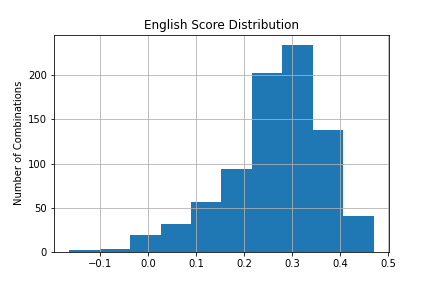
\includegraphics[width = 2in]{sections/figures/eng_score_distribution.png}}\quad
  \subcaptionbox{German}{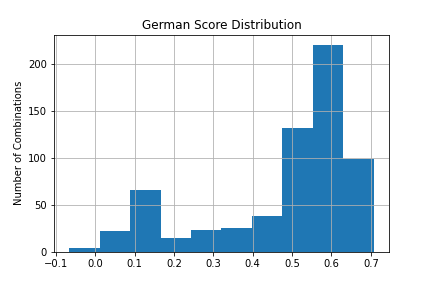
\includegraphics[width = 2in]{sections/figures/deu_score_distribution.png}}\\
  \subcaptionbox{Latin}{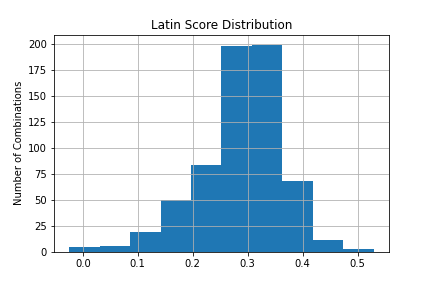
\includegraphics[width = 2in]{sections/figures/lat_score_distribution.png}}\quad
  \subcaptionbox{Swedish}{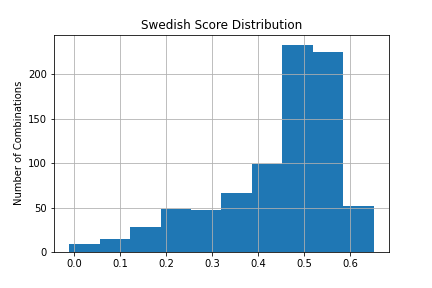
\includegraphics[width = 2in]{sections/figures/sve_score_distribution.png}}
  \caption{Distribution of $\rho$ Scores for Each Language}
  \label{fig:score-dist}
\end{figure}


The hyperparameter search successfully found model combinations that outperformed both the best teams in the SemEval task and \citet{kaiser-etal-2020-ims}’s post-hoc optimizations for both English and Latin. As seen in \autoref{tab:performance-comparison} a model was found to surpass the score of the best team in SemEval but not \citet{kaiser-etal-2020-ims} for the German language. The top-performing models and their hyperparameters are shown in \autoref{tab:top-models}. Although it is important to analyse the top results for each language separately, it is interesting to see commonalities between all four languages. The Orthogonal Procrustes alignment method seems to be the most effective for bigger datasets. For smaller datasets such as Latin, the incremental training alignment method is the most effective as the second time period model has information learned from both the first and second time period corpora. Epochs were also surprisingly low (WHY?) and lower frequency thresholds performed best as it included the maximum amount of words in the model’s vocabulary. 

\begin{table}[h]
\centering
\begin{tabular}{|l|l|l|l|} 
\cline{2-4}
\multicolumn{1}{l|}{\textbf{ }} & SemEval         & Kaiser                   & Best                      \\ 
\hline
English                         & \textit{ .422 } & \textit{ .460 }          & \textbf{\textit{ .469 }}  \\ 
\hline
German                          & \textit{ .725 } & \textit{\textbf{ .780 }} & \textit{ .706 }           \\ 
\hline
Latin                           & \textit{ .462 } & \textit{ .410 }          & \textbf{\textit{ .529 }}  \\ 
\hline
Swedish                         & \textit{ .604 } & \textit{\textbf{ .670 }} & \textit{ .651 }           \\
\hline
\end{tabular}
\caption{Top $\rho$ score comparison between SemEval-2020 Task 2 teams, \citet{kaiser-etal-2020-ims}, and results.}
\label{tab:performance-comparison}
\end{table}


\begin{table}[h]
\centering
\begin{tabular}{cccccccc} 
\toprule
\textbf{ } & \textbf{ Algorithm } & \textbf{ Alignment } & \textbf{ Vocab Size } & \textbf{ Epochs } & \textbf{ Dims } & \textbf{ Freq Threshold } & \textbf{ $\rho$ }  \\
English    & FT              & OP               & ALL (16429)      & 5                 & 300             & 10               & .469            \\
German     & W2V             & OP               & ALL (218507)     & 5                 & 25              & 5                & .706            \\
Latin      & W2V             & INC              & -                & 5                 & 10              & 10               & .529            \\
Swedish    & FT              & OP               & 5000             & 10                & 50              & 10               & .651            \\
\bottomrule
\end{tabular}
\caption{Top-performing models for each language and their parameters. WV=Word2Vec, FT=FastText, OP=Orthogonal Procrustes, INC=Incremental}
\label{tab:top-models}
\end{table}

The following analyses will show the differences in scores when the top-performing model is taken for each language and each hyperparameter is kept the same except for one hyperparameter. For example, Latin’s best model has the hyperparameters: Word2Vec, Incremental Training, 5 epochs, 10 dimensions, 10 frequency threshold. To explore the effects of the change in epochs, all the hyperparameters will remain the same except for epochs. The scores for each of these models are represented by a point in the graph where the $x$-axis is hyperparameter in question and the $y$-axis is  the Spearman $\rho$ score. These points are joined by a dotted line graph and each line represents one of the four languages. Points that are in grey are statistically insignificant where p-value > 0.05 but they are included for X (WHAT TO SAY?). Individual graphs for each language are available to examine in the APPENDIX. (WORDING) In order to extrapolate information from the data collected, the dotted lines are created in order to see trends between the points. However, it is acknowledged that if models were actually trained for each increase in the hyperparameter in question, trends in reality could show very different results. (NECESSARY BUT IS IT ALSO INVALIDATING?)

The relationship between epochs and performance raises the question of priority of performance and environmental impact. In \autoref{fig:all-epochs}, English and Swedish do not have 100-epoch models since it was deemed that their improved performance return was minimal compared to the time spent and energy consumption for training. There is a general decline in $\rho$ as epochs are increased for English, Latin, and Swedish while German had a slight increase in $\rho$ from 50 to 100 epochs. German and Latin appear to experience a similar decrease by 20 epochs but diverge after 50 epochs where German increases and Latin significantly decreases. This divergence might be attributed to the dataset size since the German corpora is much larger and there is more for the model to learn as epochs are increased. On the other hand, the Latin corpora is very limited and after 50 epochs, the decrease in $\rho$ could be additional noise being introduced to the model. Although there might still be an increase in performance when training for more than 50 or 100 epochs, lower epochs seem to be the better choice for LSC. It also is a question of priority—smaller epochs or spending more time, memory, and energy. For this hyperparameter, the option to have a smaller environmental impact compromises very little in terms of performance. 

\begin{figure}[h]
  \centering
  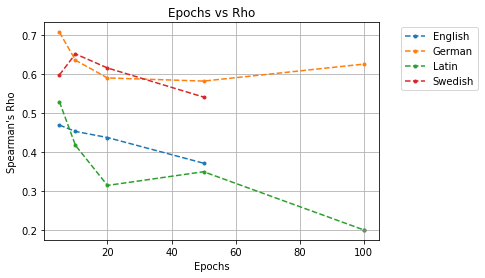
\includegraphics[width=.8\linewidth]{sections/figures/epochs_all.png}
  \caption{Change in Epochs vs. Score}
  \label{fig:all-epochs}
\end{figure}

The dimensions hyperparameter refers to the size of the vector for each word representation. Increasing vector dimensions requires a higher computational time and more memory. As expected, English performs best with higher dimensions. The 300-dimension hyperparameter is commonly used for LSC tasks (CITE?) and is usually the baseline when conducting LSC tasks on other languages due to the prevalence in studies being done in English. As seen in \autoref{fig:all-dims}, choosing higher dimensions does not necessarily result in better $\rho$ scores as it does with the English language. German, Swedish, and Latin all have higher $\rho$ scores when lower dimensions are used. Latin’s top model performed best with the lowest dimension of 10. Since the Latin corpora is very small compared to the other three languages, having less abstractions of words in the vector representations might have been more useful for the model and minimised the introduction of noise. The genre makeup of corpora is also put into question as it seems to have an effect on the vector dimensions and therefore affects performance. Swedish and German are both composed of newspaper corpora and so the same style and type of language is used. English has a mixed genre corpora and Latin is somewhere in between. Since Swedish and German models are trained on texts that have their own writing style where constructions of sentences are similar but the words have been used under many contexts, vectors with higher dimensions allow for those nuances to be learned. In comparison with Latin where the corpora consists of a wide range of texts compiled and vectors with lower dimensions allows the model to learn the usages of the words in a broader context. The genres of text being included in the corpora must be taken into consideration before choosing the vector dimensions for a model. The typical baseline of 300 dimensions, based on English results in past LSC tasks, shows not as effective on other languages. (WORDING?)

\begin{figure}[h]
  \centering
  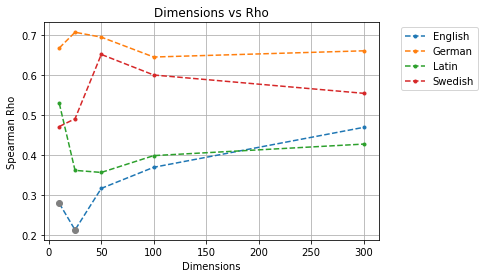
\includegraphics[width=.8\linewidth]{sections/figures/dims_all.png}
  \caption{Change in Dimensions vs. Score}
  \label{fig:all-dims}
\end{figure}

The frequency threshold hyperparameter refers to the minimum number of times a word has to appear in a corpus to be included in the model’s vocabulary. Smaller frequency thresholds will result in a larger vocabulary. Since the vocabulary is larger, memory needed will also be larger as there are more vectors to be stored and learned by the model.  \autoref{fig:all-freqs} illustrates that it is generally better to have a lower frequency threshold in order to ensure that majority of the words in a corpus is being included. German and Swedish do not have 4 points in \autoref{fig:all-freqs} as the $\rho$ scores for those model combinations were NaNs. While German performs best with the lowest frequency threshold of 5, English, Latin, and Swedish all perform better at a slightly higher frequency threshold of 10. A steady decrease in $\rho$ scores are seen as the frequency threshold increases. This is expected since a higher frequency threshold results in less words in the vocabulary and a smaller vocabulary naturally excludes words that contribute to the contextual meaning of a word. 

\begin{figure}[h]
  \centering
  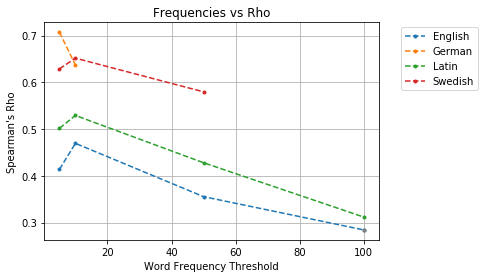
\includegraphics[width=.8\linewidth]{sections/figures/freqs_all.png}
  \caption{Change in Frequency Thresholds vs. Score}
  \label{fig:all-freqs}
\end{figure}

Two approaches were used for the orthogonal procrustes alignment method—Ryan Heuser’s Tutorial\footnote{\url{https://gist.github.com/quadrismegistus/09a93e219a6ffc4f216fb85235535faf}} and VecMap\footnote{\url{https://github.com/artetxem/vecmap}}. The former had a default of including the entire shared vocabulary of the first time period corpus and the second time period corpus during the alignment process. However, the latter included the option to indicate the size of the shared vocabulary during the alignment process. \autoref{fig:all-vocabalign} shows the effect of vocabulary size during the orthogonal procrustes alignment process on $\rho$ scores using VecMap. Latin is not included in this graph since its top-performing model used the incremental training alignment method. English and German seem to be affected similarly from this hyperparameter while Swedish experiences the opposite. German profits when the entire vocabulary (where the vocabulary size is 218, 507) is included in the alignment process and results in the top-performing model. Swedish experiences a similar increase in performance when the vocabulary size is 5000. However, the top-performing model for Swedish has a vocabulary size of 5000 and an increase in vocabulary size shows a decrease in $\rho$ scores. Although English has a significantly smaller corpora size, it also profits from the inclusion of the entire vocabulary (where the vocabulary size is 16, 429) when aligning both time period models. (NEED CRITIQUE OR CONCLUSION)

\begin{figure}[h]
  \centering
  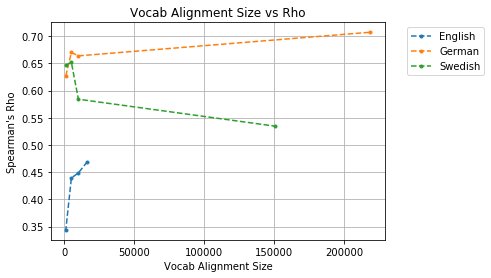
\includegraphics[width=.8\linewidth]{sections/figures/vocabalignment_all.png}
  \caption{Vocabulary Size in Orthogonal Procrustes Alignment vs. Score}
  \label{fig:all-vocabalign}
\end{figure}

\subsection{POS}

Every model trained was also evaluated by creating smaller target word lists based on each word’s POS-tag. For each language’s target word list, words have been manually annotated FOOTNOTE THANKS POS-tagged as either a noun (NN), verb (VB), or adjective (ADJ). The target word list breakdown for each language is seen in \autoref{fig:target-postags}. Nouns are much more prevalent in the target word lists and so conclusions made for nouns are much more concrete (BETTER WORD, reliable? sure? Interpretable? Or conclusions made for nouns are more meaningful on the grounds of…) compared to conclusions made for verbs and adjectives. Control words within each POS-tag are also shown in FIGURE POS-TAGS through a lighter colour respective of its POS-tag. With already a smaller ratio and an addition of control words that have 0 as a cosine distance, a $\rho$ score of 1 can sometimes be more easily attained since it is calculated by rank. For example, if there are only 2 words for A LANGUAGE adjectives and one is a control word, a model’s chances of obtaining a perfect Spearman $\rho$ score of 1 is very high. 


\begin{figure}[h]
  \centering
  \subcaptionbox{English}{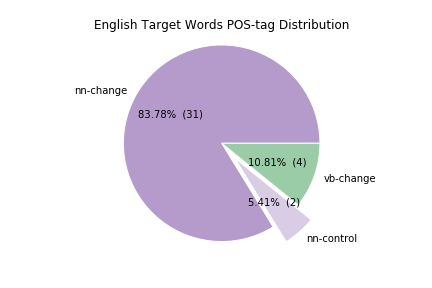
\includegraphics[width = 3in]{sections/figures/eng-pos-target-control.png}}\quad
  \subcaptionbox{German}{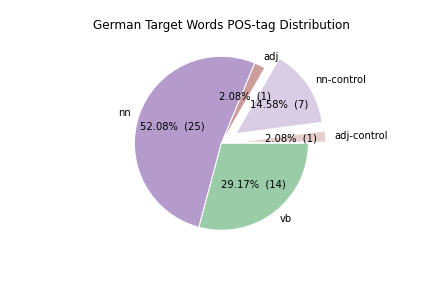
\includegraphics[width = 3in]{sections/figures/deu-pos-target-control.png}}\\
  \subcaptionbox{Latin}{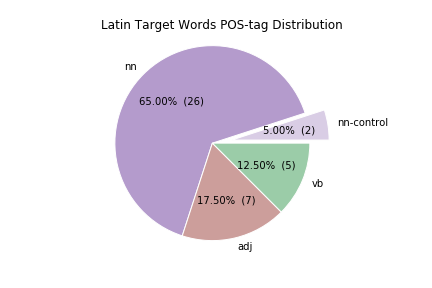
\includegraphics[width = 3in]{sections/figures/lat-pos-target-control.png}}\quad
  \subcaptionbox{Swedish}{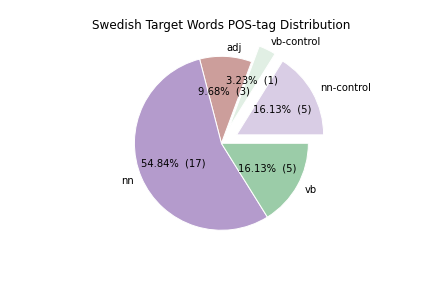
\includegraphics[width = 3in]{sections/figures/sve-pos-target-control.png}}
  \caption{Target Word POS-tag Distribution for Each Language}
  \label{fig:target-postags}
\end{figure}
